% \section{Introduction}
% Epilepsy is a neurological condition predominantly characterized by the protracted recurrence of
% seizures.

% These temporary disturbances of neurological brain function affecting over 50 million
% people worldwide have been attributed to various causes, such a stroke, head trauma, and infections.
% However, patients may nonetheless present seizures of an unknown cause at the clinic, with resection
% of epileptic tissue serves as a last line of defence.

% One avenue of research has focused on the SCNA1 gene, a sodium channel gene
% with a history of mutations associated with epilepsy. For instance, mutants exhibit subtle
% differences in voltage-gated sodium ion channel density along the cellular membrane. These changes
% in channel density have been thought to underlie the physiological disturbance that results in
% abnormal neurological functioning found in epilepsy. Here, we utilised two previously developed
% models of SCNA1 mutations, the Q1489K and L1649Q variants, to gain a greater understanding of the
% specific downstream cellular signalling mechanisms that are affected by changing the density of
% mutated membrane sodium channels.

\section{Signalling Models}
We used two deterministic computational models to investigate the effects of sodium channel
mutations on the downstream signalling dynamics within the neuron. The first model uses a
Hodgkin-Huxley framework to determine the voltage and calcium levels at the soma and dendrite based
on the channel characteristics described in Hay et al. \cite{hay2011models}.

Using this model, we stimulated neurons at the soma and recorded the voltage and calcium levels at
the dendrite for both a control neuron and neurons with increasing percentages of mutated sodium
channels. We recorded the difference in peak calcium levels between the control and mutated cases
for use as input to the second model.

The second model is a signalling model of the signalling cascade following calcium influx into the
neuron, based on Jedrzejewska-Szmek et al. \cite{jȩdrzejewska2017beta}. It should be noted that
while Jedrzejewska-Szmek et al. used a multi-compartmental model, we use a well-mixed model for
simplicity. We use model two to find the GluR (AMPAR) levels modulating the calcium influx based on
the readouts from model one.

The effect of mutations Q1481K and L1649Q in the SCN1A gene was studied. The mutations were
included by modifying the sodium conductance and gating variables in the multicompartmental L5PC
model for both the soma and the apical dendrite. The altered parameters for the variants were taken
from \cite{maki2016functional}.

\section{Signalling Results}
% Neurons with mutated sodium channels depart from typical neuron dynamics in regard to voltage,
% calcium dynamics and GluR levels.
Both mutations show substantial jump in dendritic membrane voltage, as seen in \cref{fig:volt}. We
will focus on mutation one, because lower fractions of mutated sodium channels can have a
significant effect on neuronal dynamics. Mutation one exhibit ultrasensitivity towards increasing
fraction of mutated channels. This manifests itself as a switch-like behaviour, as seen in
\cref{fig:ultra}. Therefore, once a neuron hits this threshold, calcium levels will increase
significantly. There is a similar effect in GluR dynamics, as seen in \cref{fig:GluR}.

% For the two SCNA1 mutations of interest, we see that mutation 1 has a substantial jump in dendritic
% membrane voltage at 10\% mutation, while mutation 2 shows a jump at 15\% mutation, see
% \cref{fig:volt}. We will focus on mutation one, because a lower fraction of mutated sodium channels
% can have a significant effect on neuronal dynamics.

% Looking at the maximum calcium concentration at the dendrite, we can clearly see that mutation one
% exhibits ultrasensitivity towards increasing channel percentages. This switch-like behaviour occurs
% around 7.5\% mutation, see \cref{fig:ultra}. Therefore, once a neuron hits this threshold it will
% experience a significant increase in calcium levels. There is a similar trend in GluR dynamics, see
% \cref{fig:GluR}. We consider the temporal dynamics of single phosphorylated GluR, and see that there
% is a similar jump between 5\% and 10\% mutation.  Initially GluR rises to a basal concentration,
% then at a critical time point calcium dynamics begin to influence GluR. We see that the increase in
% 10-20\% mutation leads to about twice the increase in GluR compared to the control and 5\% mutation. 

\section{Limitations in our signalling approach}

% TODO: Reduce this to two lines!!!!!!!

%%% Future work
Future work should take into consideration the morphology of the modelled neurons, as their terminal
connections could affect their afferent networks differently depending on the multitude of terminal
synapses.


% TODO: What does this mean? Where the neuron is stimulated?
Another consideration is the location and nature of input stimulation. For example, our method could
be contrasted with simulated input from an upstream neuron, which may reflect the network in which a
neuron is situated more accurately.

Furthermore, stimulation at the terminals could reveal the
voltage dynamics of our simulated mutant neurons in a way that would make their output to downstream
neurons measurable. For instance, stimulating at the dendrite of a mutant 1 (Q1489K) neuron could
reveal a greater voltage at the terminals, which may determine terminal output of vesicle release.

% TODO: Make this into subfigures.
% \begin{figure}[!!h]
%     \centering
%     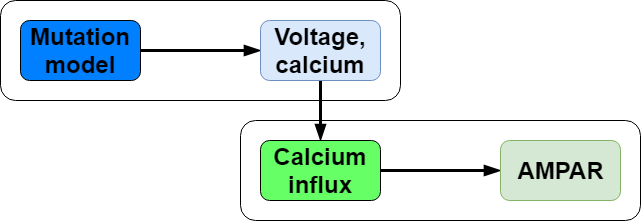
\includegraphics[width=\textwidth]{images/schematic.png}
%     \caption{\textbf{Model Design} We combine two signalling models to investigate the impact of
%     sodium channel mutations on calcium and AMPAR (GluR) dynamics.}
%     \label{schematic}
% \end{figure}

\begin{figure}[!!h]
    \centering
    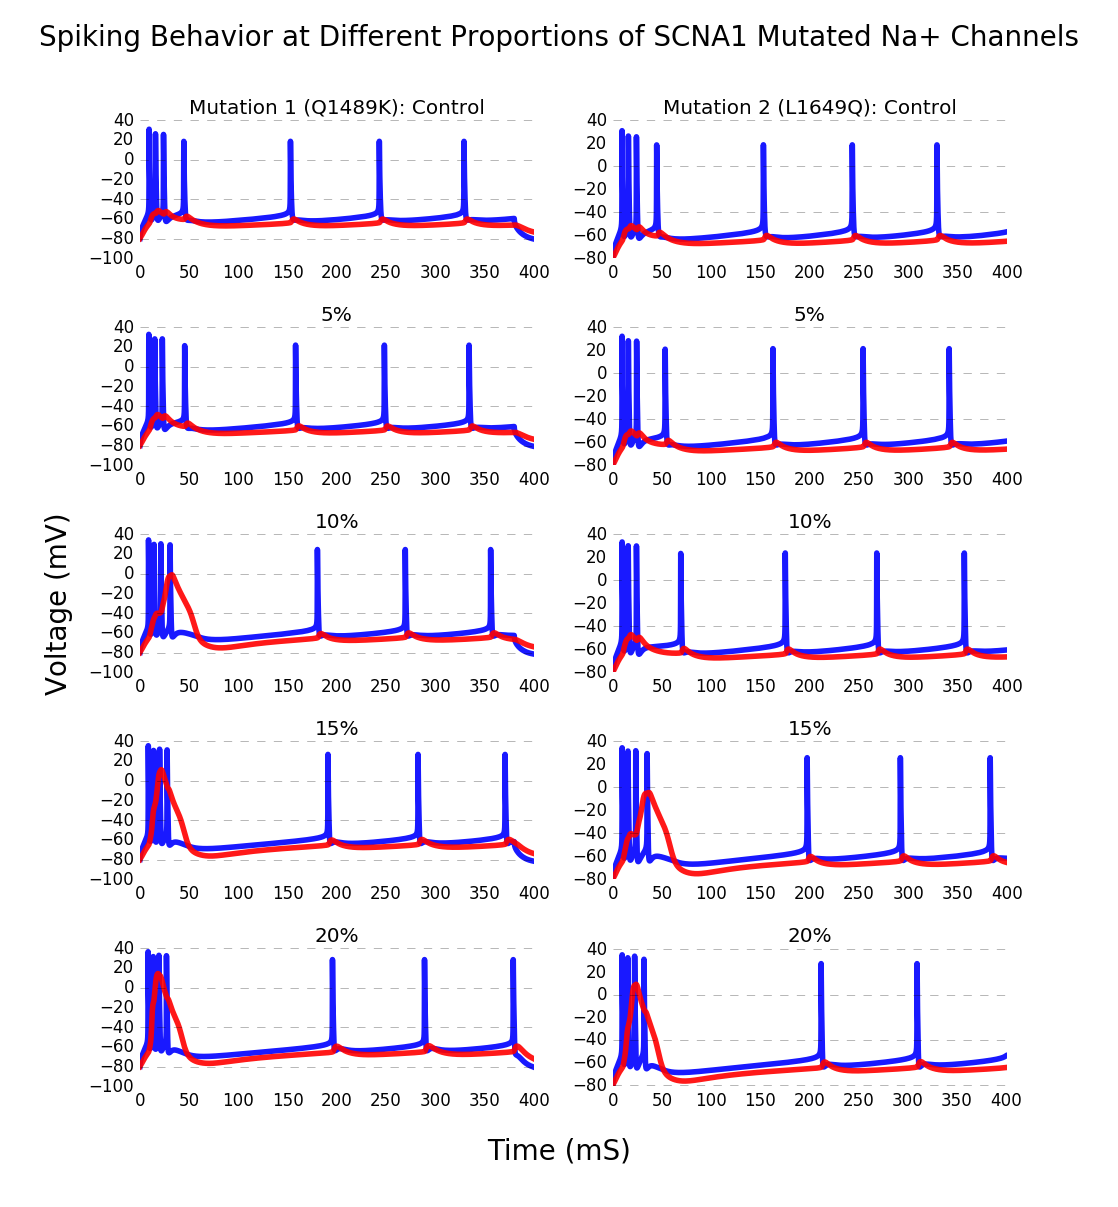
\includegraphics[width=1\textwidth]{images/spikes_all.png}
    \caption{\textbf{Voltage dynamics for two mutations} We model neurons with 0-20\% mutated sodium
    channels for two different types of mutations}
    \label{fig:volt}
\end{figure}

\begin{figure}[!!h]
    \centering
    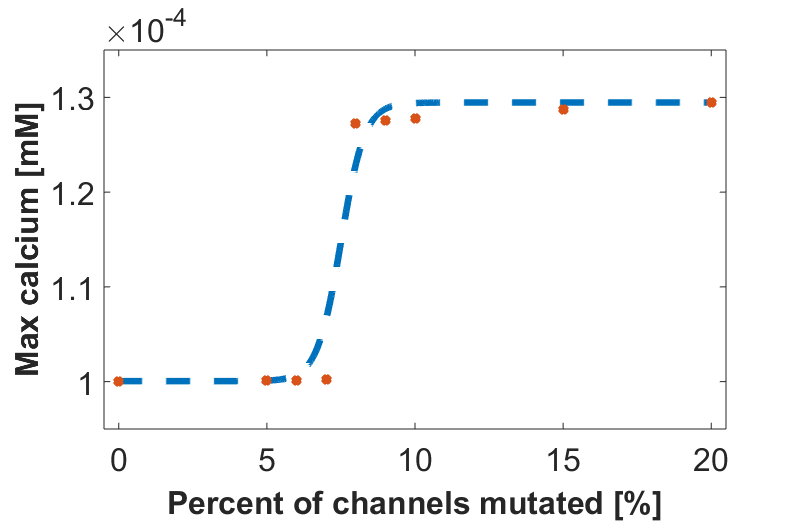
\includegraphics[width=1\textwidth]{images/ultraGraphSomaStim.png}
    \caption{\textbf{Calcium dynamics at the dendrite} We stimulated the neuron at the soma and
        recorded calcium readout at the dendrite. We found for mutation 1 that the calcium
        dependence of mutation percentage showed ultrasensitivity. For illustrative purposes, we
        have fit the data with a hyperbolic tangent to show the switch-like behavior around 7.5\%
        mutation.}
    \label{fig:ultra}
\end{figure}

\begin{figure}[!!h]
    \centering
    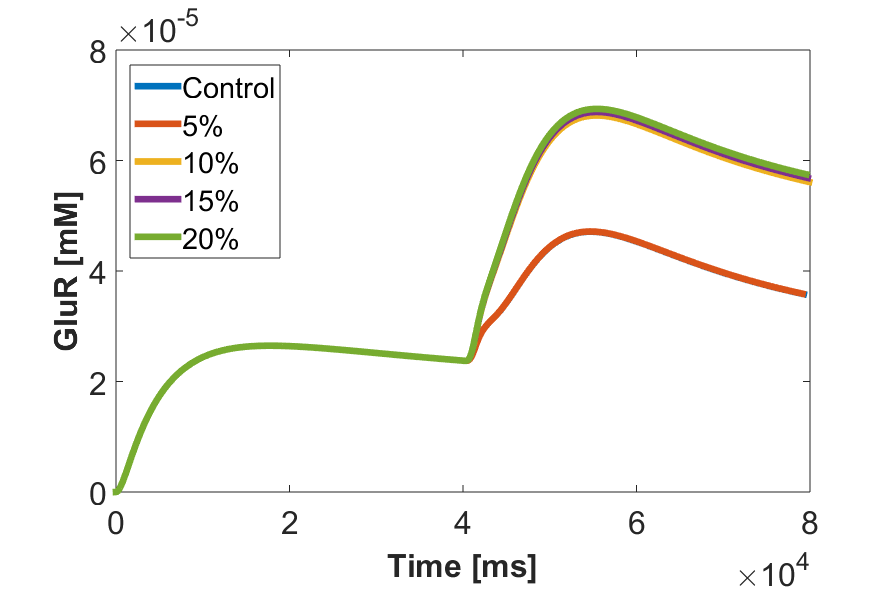
\includegraphics[width=1\textwidth]{images/GluRTimeSomaStim.png}
    \caption{\textbf{GluR dynamics} We modulate calcium influx into our signaling model based on the
        output of the voltage model to get our final readout of GluR. We see that all mutation
        levels show similar dynamics until a distinct time point in which 10\%, 15\%, and 20\%
        mutation all increase relative to the control.}
    \label{fig:GluR}
\end{figure}

% Using a combination of voltage and signaling models, we investigated the effects of sodium channel
% mutations characteristic of epilepsy. We found that by changing the percentage of sodium channels
% affected by this mutation, we can see departures from typical neuronal dynamics in regards to
% voltage, calcium dynamics, and GluR levels. For the two SCNA1 mutations of interest, we see that
% mutation 1 has a substantial jump in dendritic membrane voltage at 10\% mutation, while mutation 2
% shows a jump at 15\% mutation, see Fig. \ref{volt}.

% In essence, a cortical neuron in a laminar structure may have limited spread of
% overexcitation in comparison to a localized, inhibitory medium spiny neuron located in the striatum.
